We compared two different base classification models to analyze their ability to learn from these small handshape datasets; Prototypical Networks \cite{protonet} and DenseNet \cite{densenet}. Prototypical Networks is a model that was designed explicitly to deal with small sample sizes. On the other hand, DenseNet is currently a state of the art model in image classification with convolutional neural networks, and while it has not been explicitly designed for small datasets, it has shown exceptional performance in many different tasks. 

In the case of DenseNet, we also experiment using Model-Agnostic Meta-Learning (MAML) \cite{DBLP:journals/corr/FinnAL17} and Transfer Learning \cite{tan2018} training techniques, in addition to the traditional training process. 

Transfer Learning is a well known technique to jump-start the training of neural networks for a problem A using datasets from a similar problem B. The weights of a network trained on B are used as initial weights in the training of the network for A. Retraining the network for A is called finetuning, and may retrain only a subset of the weights of the network. However, it still may require large amounts of data for the finetuning phase.

Finally, MAML is a meta-learning technique for few-shot learning, that involves learning subtasks. In this context, each subtask corresponds

In the following subsections we describe in more detail each of these models.

\subsubsection{Wide-DenseNet}

We selected a DenseNet based architecture as it is a state of the art model in many domains and can handle small datasets with low error rate \cite{pmlr-v80-pham18a}.

DenseNet \cite{densenet} works by concatenating the feature-maps of a convolutional block to the feature-maps of all the previous convolutional blocks and using the resulting set of feature-maps as input for the next convolutional block. In this way, each convolutional block receives all the collective knowledge of the previous layers maintaining the global state of the network which can be accessed.

We employed a variation on DenseNet called Wide-DenseNet which follows the strategy used by wide residual networks \cite{He2015DeepRL}. Wide-DenseNet consists on decreasing the depth of the network and increasing the width of the layers. This way the model can be trained faster by optimizing feature reuse and obtain higher accuracy.

Additionally, we use Squeeze and Excitation blocks (SE blocks) \cite{Hu2017SqueezeandExcitationN} to improve the performance of the DenseNet model. Convolutional networks construct informative features by fusion both spatial and chanel-wise information within local receptive fields at each layer. SE blocks focus on  channel-wise information, improving the quality of the representations produced by the network by modeling the interdependency between channels to perform feature recalibration. SE blocks can be included in any model that uses convolutional layers to improve its performance at low computational cost. We use SE blocks between dense and transition blocks, see figure \ref{fig:densenet}.

\begin{figure*}[!ht]
    \centerline{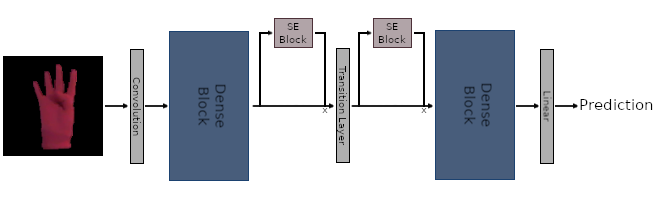
\includegraphics[width=0.85\textwidth]{images/background/densenet.png}}
    \caption{DenseNet using 2 dense blocks and SE blocks.}
    \label{fig:densenet}
\end{figure*}

\subsubsection{Transfer Learning} \label{models:tl}

Gathering new training data for deep neural networks can be an expensive and time consuming task. Transfer learning provides a way to utilize already available data from a source domain and transfer the acquired knowledge from this source domain to a target domain. By doing transfer learning we can obtain much better initializations of the parameters of the model before training in the target domain. 

In the past, transfer learning has been used for handshapes, sign language and gesture recognition \cite{farhadi2007}\cite{quiroga2017study}\cite{allard2017} demonstrating the advantages of this technique. 

In this work,  we are doing Network-based \cite{tan2018} transfer learning. In this type of transfer learning a part of the network pretrained on the source domain is reused for the training in the target domain. The objective is for the neural network to acquire abstract information from the source domain and transfer this knowledge to the target task.

To obtain a good performance from transfer learning it is commonly needed for the source dataset to be larger than the target dataset. Since the information extracted from the target dataset has a higher value than the information from the source dataset, the data from the target dataset will be more helpful in fitting the target task. In addition to this, it is important for the source domain to be well related to the target domain. If the relation between both domains differ too much it is possible to get a negative transfer which can diminish the performance obtained by using transfer learning to the point of obtaining less performance by applying it \cite{weiss2016}.

\subsubsection{Model-Agnostic Meta-Learning} \label{sec:models:maml}

Like Prototypical Networks, Model-Agnostic Meta-Learning (MAML) \cite{DBLP:journals/corr/FinnAL17} is a technique designed to tackle the problem of few-shot learning. MAML learns how to improve a model so that it can learn a new task in only a few steps by training on many different tasks, commonly phrased as learning to learn. MAML does this by learning over multiple tasks and updating the parameters of the models based on the improvement obtained after training on each task.

More formally, given a set of tasks $T$ each consisting of a loss function $L$ and a set of elements with their corresponding labels. MAML requires a distribution over tasks $p(T)$ that we want to adapt to. Given those distributions, we proceed with the next two steps, task training and meta training. In the task training we sample $K$ tasks. For each task $T_i$, the model is trained on a set of elements extracted from the task distribution using the loss function $L_i$ belonging to $T_i$. With the updated parameters the model is then tested on new data from $T_i$. Once tested on each task the loss obtained from these tests will be added and utilized as loss for the initial model on the meta training obtaining a new initial model with better initial parameters that will grant a bigger improvement for each task on fewer steps.

We made some modifications on the original MAML to work with bigger datasets in a supervised way. Each task $T_i$ is split in 2 subsets, a training subset $Tt$ and a meta training subset $Tm$. The subsets are composed of datasets $D={x,y}$ where $x$ is an image and $y$ the label of that image. Each subset has an equal size $b$ and its labels are mirrored $y\in Tt \iff y\in Tm$. Each dataset with size $n$ has $n/2b$ tasks $T$. We consider our model as a function $f_\theta$ with parameters $\theta$. In each training iteration $\theta$ will change to $\theta'$. Each iterations consists of 2 steps, a training and a meta training step. In the training step we start by storing the value of $\theta$ in $\theta'$, then $\theta$ is updated to fit $Tt_i$. In the meta training step the new $\theta$ is used to calculate the gradients with $Tm_i$ : $\nabla L_i(  f_\theta(Tm_i))$ and these gradients are applied to $\theta'$ finishing the iteration. 

\begin{algorithm}[!h]
\caption{Model-Agnostic Meta-Learning for Few-Shot Supervised Learning}
\SetAlgoLined
\KwIn{A set of tasks T }
 Initialize $\theta$\;
 \While{not done}{
  \For{$T_i$ in $T$}{
   Save the parameters $\theta$ in $\theta'$\;
   Train $\theta$ using the training subset: $\theta = \theta -  \alpha \nabla L_i( f_\theta(Tt_i))$ \;
   Get the gradients using the meta training subset: $\nabla L_i(  f_\theta(Tm_i))$ \;
   Apply the gradients to $\theta'$: $\theta' = \theta' - \alpha \nabla L_i( f_\theta(Tm_i))$\;
  }
 }
 Train $f_\theta$ in the objective dataset with less samples
\end{algorithm}

\subsubsection{Prototypical Networks}
\label{models:protonet}

Prototypical Networks \cite{protonet} is a meta-learning model for the problem of few-shot classification, where a classifier must generalize to new classes not seen in the training set, given only a small number of examples of each new class. The ability of an algorithm to perform few-shot learning is typically measured by its performance on n-shot, k-way classification tasks. First a model is given a set of query samples Q belonging to a new, previously unseen class. Then, it receives a support set, S, consisting of n examples, each from k different unseen classes. Finally, the algorithm has to determine the classes of Q, given the samples of S, see figure \ref{fig:protonet:handshape}.

\begin{figure}[!ht]
    \centerline{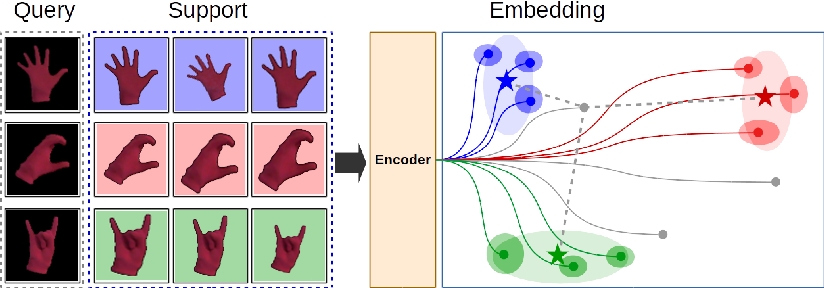
\includegraphics[width=1.0\columnwidth]{images/background/protonets.png}}
    \caption{Prototypical Networks given a set of query samples and support set}
    \label{fig:protonet:handshape}
\end{figure}

Prototypical Networks apply an inductive bias in the form of class prototypes to achieve impressive few-shot performance. The key assumption is the existence of an embedding in which samples from each class cluster around a single prototypical representation which is simply the mean of the individual samples. This idea streamlines n-shot classification in the case of $n > 1$ as classification is simply selecting the label of the closest class prototype, see figure \ref{fig:protonet}.

Schemes for few shot classification tasks like Prototypical Networks can also be of use for training small datasets.

\begin{figure}[!ht]
    \centerline{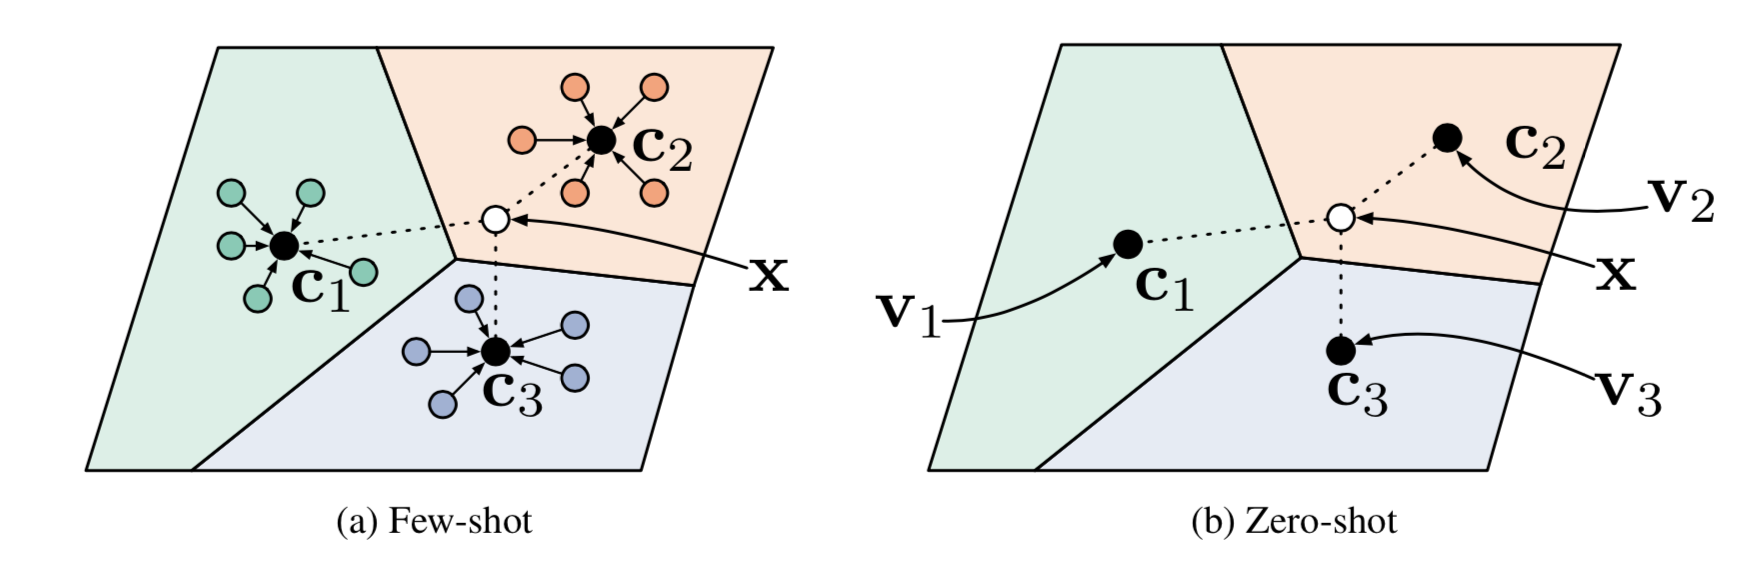
\includegraphics[width=1.15\columnwidth]{images/background/prototypical-networks.png}}
    \caption{Prototypical networks in the few-shot and zero-shot scenarios. \textbf{Left}: Few-shot prototypes
    $\mathbf{c}_k$ are computed as the mean of embedded support examples for each class. \textbf{Right}: Zero-shot prototypes $\mathbf{c}_k$ are produced by embedding class meta-data $\mathbf{v}_k$. In either case, embedded query points are classified via a softmax over distances to class prototypes.}
    \label{fig:protonet}
\end{figure}
